%!TEX root = TQFTnotes.tex
%%%%%%%%%%%%%%%%%%%%%%%%%%%%%%
\chapter{Spherical fusion categories}\label{c:spherical}

In this chapter we will study some algebraic properties of spherical fusion
categories. We will use these results in the next chapter for constructing
a lattice extended TQFT, the Turaev--Viro theory.

Throughout this chapter, $\calC$ is a spherical fusion category over an
algebraically closed field $\kk$ of characteristic zero (see \deref{d:pivotal},
\deref{d:spherical}).

We denote by $\OC$ the set of isomorphism classes of simple objects in $\calC$;
by definition of a fusion category, it is a finite set, and we will choose a
representative $X_i\in \calC$ for every $i\in \OC$. Abusing the language, we
will write things such as $\bigoplus_{X\in \OC} \End(X)$ instead of
$\bigoplus_{i\in \OC}\End(X_i)$. All our formulas will be independent of the
choice of representatives.

It is known that any pivotal category is monoidally equivalent to a strictly
pivotal category, i.e., a category in which $V^{**}=V$. Therefore in most
formulas below we will suppress $\de$, in the same way as when working with
monoidal categories, we frequently suppress the associativity isomorphisms.



%%%%%%%%%%%%%%%%%%%%%%%%%%%%%%%%%%%%%%%%%%%%%%%%
\section{Graphical calculus}\label{s:graphical}
In the previous chapters, we had already used graphical presentations
of morphisms in a monoidal category. However, until now it was informal:
it was only used as an illustration of our constructions and proofs.
In this section, we will finally make some precise statements about such
graphical presentations.

The idea of using such graphics is quite old; it seems that it was first
suggested by Penrose, and then made popular by Joyal and Street
\ocite{joyal-street}, \ocite{joyal-street2} and by Reshetikhin and Turaev
\ocite{reshetikhin-turaev}. Our exposition follows the recent book
\ocite{turaev-virelizier}*{Chapter 2}, which provides the cleanest exposition
of these results. Note, however, that in that book their convention is that
graphs should be read ``from the bottom up'': incoming objects are shown at the
bottom, and outgoing, at the top. We use the opposite convention, so we
slightly modify their definitions.

Let $\calC$ be a pivotal category. Following \ocite{turaev-virelizier}, we
define a $\calC$-colored \emph{Penrose diagram} to be the following data:
\begin{itemize}
  \item a finite collection of non-intersecting ``boxes'', i.e., rectangles
  with vertical/horizontal sides in the strip $\R\times [0,1]$
  \item a finite collection of non-intersecting smooth directed arcs (embedded
  intervals) and directed circles (images of $S^1$) in the strip $\R\times
  [0,1]$. Endpoints of arcs are all distinct and can lie
  either on the horizontal sides of boxes or the top and bottom of the strip,
  i.e., lines $\R\times\{1\}$, $\R\times \{0\}$. At the endpoints, the lines
  must be transversal to the horizontal lines. Other than the endpoints, arcs
  and circles do not intersect the boxes or top and bottom lines.
  \item coloring, i.e., assignment of an object of $\calC$ to every arc or
  circle, and assignment of a morphism in $\calC$ to every box. Namely, if
  $A_1, \dots, A_k$ are the colors of the arcs ending at the top side of a box,
  and $B_1, \dots, B_m$ are colors at the bottom of the box (both read left to
  right), then the box must be colored by a morphism
  $$
    \ph\in \Hom_\calC(
      A_1^{\eps_1}\otimes\dots\otimes A_k^{\eps_k},
      B_1^{\eps'_1}\otimes\dots\otimes B_m^{\eps'_m}
    )
  $$
  where
  \begin{equation}\label{e:signed-object}
    A_i^{\eps_i} =\begin{cases}
                 A_i, & \text{if the corresponding arc is directed downward}\\
                 A_i^* &\text{otherwise}
                 \end{cases}
  \end{equation}
  and similarly for $B$'s, see \firef{f:graphical-morphism2}.
\end{itemize}
\begin{figure}[h]
  \centering
  \begin{tikzpicture}
    \node[morphism_sq, minimum width=2cm] (ph) at (0,0) {$\ph$};
    %% top
    \node[label=above:$A_1$] (A1) at (-0.7,1){};
    \node[label=above:$A_2$] (A2) at (0,1){};
    \node[label=above:$A_3$] (A3) at (0.7,1){};
    \draw[->] (A1)-- (A1|-ph.north);
    \draw[<-] (A2)-- (A2|-ph.north);
    \draw[->] (A3)-- (A3|-ph.north);
    %% bottom
    \node[label=below:$B_1$] (B1) at (-0.4,-1){};
    \node[label=below:$B_2$] (B2) at (0.4,-1){};
    \draw[->] (B1)-- (B1|-ph.south);
    \draw[<-] (B2)-- (B2|-ph.south);
    %% eqn
    \node[right] at (2,0) {$\ph\colon A_1\otimes A_2^*\otimes A_3\to
    B_1^*\otimes
    B_2$};
  \end{tikzpicture}
  \caption{Graphical notation for a morphism in a monoidal category.}
  \label{f:graphical-morphism2}
\end{figure}

An example of such a diagram is shown in \firef{f:diagram2}.

\begin{figure}[ht]
  \centering
  \begin{tikzpicture}
    % top and bottom
    \draw[blue] (-4, 2.2)--(3,2.2);
    \draw[blue] (-4, -2.2)--(3,-2.2);
    \coordinate (bot) at (0,-2.2);
    % morphism boxes
    \node[morphism_sq] (g) at (0,0.7) {$\ph$};
    \node[morphism_sq] (k) at (0,-1.3) {$\psi$};
    \node[morphism_sq] (h) at (2,-0.4) {$\al$};
    % --- box k: two strands down to bottom
    \draw[midarrow] (k.295) |- (bot) node[above right] {$R$};
    \draw[midarrow] (k.245|-bot) -- (k.245) node[pos = 0.5, left] {$P$};

    % --- box g: V in (top), X loop (left), Z out (bottom, to k) ---
    \draw[midarrow] (0,2.2) -- (g.north);
    \node[above] at (0,2.2) {$V$};
    \draw[midarrow] (k.north) -- (g.south);
    \node[right] at (0,-0.5) {$Z$};
    \draw[midarrow] (-0.15,0.95) to[out=90,in=90,looseness=2] (-1,0.7)
                      to [out=-90, in=-90, looseness=2] (-0.15, 0.45);
    \node[left] at (-0.27,1.5) {$X$};
    % --- box h: B in (top), A out (bottom), Y in ---
    \draw[midarrow] (2,2.2) -- (h.north);
    \node[right] at (2,0.9) {$B$};
    \draw[midarrow] (h.south) -- (2,-2.2);
    \node[right] at (2,-1.5) {$A$};
    \draw[midarrow] (0.2,0.45) to[out=-90,in=90] (h.110);
    \node[above] at (1.0,0.15) {$Y$};
    % --- a strand colored W, with a rigidity-style zigzag ---
    \draw[midarrow=0.15] (-1.95,-2.2) -- (-1.95,-0.4)
                    arc(0:180:0.15) arc(0:-180:0.15) -- (-2.55,2.2);
    \node[left] at (-2.55,0.4) {$W$};
    % --- a strand colored U, both ends on the top line ---
    \draw[midarrow=0.2] (-3.5,2.2) to[out=-90,in=180] (-3.15,1.55)
                    to[out=0,in=-90] (-2.8,2.2);
    \node[below] at (-3.15,1.55) {$U$};
    % --- a directed circle colored X ---
    \draw[midarrow=0.25] (-1.2,-1.95) arc(-90:270:0.33);
    \node[above] at (-1.2,-1.3) {$X$};
  \end{tikzpicture}
  \caption{An example of $\calC$-colored diagram}\label{f:diagram2}
\end{figure}



For such a diagram $\Gamma$, we can define objects $F_\ttop(\Gamma)$,
$F_\bbot(\Gamma)\in \calC$ by taking the tensor product of colors of arcs with
endpoints on the top horizontal line $\R\times\{1\}$ (respectively,
$\R\times\{0\})$, with the same sign convention as in \eqref{e:signed-object}. Our
goal is to define, for any such diagram $\Gamma$, a morphism $F(\Gamma)\colon
F_\ttop(\Gamma)\to F_\bbot(\Gamma)$ in $\calC$.

To do that, note that for such diagrams (or, to be precise, for isotopy classes
of diagrams), we can define two operations.

First, if $\Gamma_1, \Gamma_2$ are diagrams such that the top of $\Gamma_2$
matches the bottom of $\Gamma_1$, we can ``stack'' them, placing $\Gamma_1$ on
top of $\Gamma_2$ and then rescaling vertically; we will denote this
composition $\Gamma_2\circ\Gamma_1$. As with gluing cobordisms, this requires
smoothing the resulting joined arcs, which is well defined on the set of isotopy
classes.

Second, we can define the tensor product $\Gamma_1\otimes \Gamma_2$ by placing
$\Gamma_2$ on the right of $\Gamma_1$ in the same strip.

\begin{figure}[ht]

  \begin{tikzpicture}[vcenter]
  %\draw (0,0)--(2.5,0); %top
  %\draw (0,-1.5)--(2.5,-1.5); %top
  \node at (-1.2, 0) {$\Gamma_2\circ \Gamma_1=$};
  \node[morphism_sq, minimum width = 1cm] at (0, 0.25) {$\Gamma_1$};
  \node[morphism_sq, minimum width = 1cm] at (0, -0.25) {$\Gamma_2$};
  \end{tikzpicture}
\qquad\qquad
  \begin{tikzpicture}[vcenter]
  %\draw (0,0)--(2.5,0); %top
  %\draw (0,-1.5)--(2.5,-1.5); %top
  \node at (-1.2, 0) {$\Gamma_1\otimes \Gamma_2=$};
  \node[morphism_sq, minimum width = 1cm] at (0, 0) {$\Gamma_1$};
  \node[morphism_sq, minimum width = 1cm] at (0.8, 0) {$\Gamma_2$};
  \end{tikzpicture}

\caption{Composition and tensor product of diagrams}
\end{figure}





\begin{theorem}\label{t:graphical-calculus1}
  Let $\calC$ be a pivotal category. Then
  there is a unique way to assign to each $\calC$-colored diagram $\Gamma$ a
  morphism $F(\Gamma)\colon F_\ttop(\Gamma)\to F_\bbot(\Gamma)$ such that
  \begin{enumerate}
    \item $F(\Gamma)$ only depends on isotopy class of $\Gamma$
    \item $F(\Gamma_2\circ \Gamma_1)=F(\Gamma_2) F(\Gamma_1)$
    \item $F(\Gamma_2\otimes \Gamma_1)=F(\Gamma_2)\otimes F(\Gamma_1)$
    \item For a diagram that consists of a single box colored by $\ph$ as in
    \firef{f:graphical-morphism2}, $F(\Gamma)=\ph$
    \item For elementary diagrams \textup{(}interval, cap, cup\textup{)}, the values of $F$ are
    as shown in \firef{f:graphical-basic}.
  \end{enumerate}
\end{theorem}
\begin{figure}[ht]
  \begin{tikzpicture}
    % ev
    \begin{scope}
    \draw[midarrow] (0.4,0) arc (0:-180:0.4);
    \node at (0, -0.1){$X$};
    \node[right,scale=0.9] at (0.8,-0.15)
        {$\ev_X\colon X^*\otimes X\to
    \one$};
    \end{scope}
    % \tilde ev
    \begin{scope}[yshift =-1cm]
    \draw[midarrow] (-0.4,0) arc (-180:0:0.4);
    \node at (0, -0.1){$X$};
    \node[right,scale=0.9] at (0.8,-0.15)
       {$\ev_{X^*}\circ (\de_X\otimes 1_{X^*})\colon X\otimes X^*\to \one$};
    \end{scope}
    % coev
    \begin{scope}[yshift =-2cm]
    \draw[midarrow] (0.4,-0.4) arc (0:180:0.4);
    \node at (0, -0.25){$X$};
    \node[right,scale=0.9] at (0.8,-0.15)
       {$\coev_{X}\colon \one \to X\otimes X^*$};
    \end{scope}
    % tilde coev
    \begin{scope}[yshift =-3cm]
        \draw[midarrow] (-0.4,-0.4) arc (180:0:0.4);
    \node at (0, -0.25){$X$};
    \node[right,scale=0.9] at (0.8,-0.15)
       {$(\id \otimes \de^{-1}_X)\coev_{X^*}\colon \one \to X^*\otimes X$};
    \end{scope}
    \begin{scope}[xshift =-3cm]
    \draw[midarrow] (0,0) --(0,-0.8);
    \node[left] at (0, -0.4){$X$};
    \node[right,scale=0.9] at (0.3,-0.4)
       {$\id_X$};
    \end{scope}
    \begin{scope}[xshift =-3cm, yshift=-2cm]
    \draw[midarrow] (0,-0.8) --(0,0);
    \node[left] at (0, -0.4){$X$};
    \node[right,scale=0.9] at (0.3,-0.4)
       {$\id_{X^*}$};
    \end{scope}
  \end{tikzpicture}

  \caption{Morphisms corresponding to elementary
    diagrams.}\label{f:graphical-basic}
\end{figure}

Note that while in the definition of a Penrose diagram we require that boxes
are oriented vertically, the isotopy is allowed to rotate the boxes (by
multiples of 360 degrees).

This theorem is a reformulation of \ocite{turaev-virelizier}*{Theorem 2.6}; we
refer the reader to that book for a proof. It can
be restated as follows. Let $\Diag(\calC)$ be the category whose objects are finite
sequences $\mathbf{A}=((A_1, \eps_1), \dots, (A_k, \eps_k))$, where $A_i$ are
objects of $\calC$ and $\eps_i=\pm 1$, and morphisms $\mathbf{A}\to \mathbf{B}$
are isotopy classes of $\calC$-colored diagrams with colors $A_1, \dots, A_k$ at
the top and colors $B_1, \dots, B_m$ at the bottom and signs $\eps$ are
determined by the orientation of the corresponding arcs as in
\eqref{e:signed-object}. The stacking and tensor product operations defined
above show that it is a monoidal category, with unit object given by empty
collection of objects of $\calC$. Then we can restate
\thref{t:graphical-calculus1} as follows.

\begin{theorem}\label{t:graphical-calculus2}
  The correspondence shown in \firef{f:graphical-basic} can be uniquely extended to
  a monoidal functor $F\colon \Diag(\calC)\to \calC$.
\end{theorem}


In particular, for a closed diagram $\Gamma$ (i.e., with empty top and empty
bottom) the above theorem defines $F(\Gamma)\in \End_\calC(\one)$. If $\calC$
is a tensor category, so that $\End(\one)=\kk$, this gives a numerical invariant
of a diagram.

This theorem makes it possible to give graphical proofs of various equalities:
in order to show that two morphisms, defined by $\calC$-colored diagrams, are
equal, it suffices to show that the diagrams themselves are isotopic. Such
proofs are much easier to follow than algebraic arguments.






%%%%%%%%%%%%%%%%%%%%%%%%%%
\section{Dimensions in a spherical category}\label{s:spherical-basic}

As before, let $\calC$ be a spherical fusion category.
Recall that by the Schur lemma (\leref{l:schur}),
for any simple $X$, we have $\End(X)=\kk$.

For an object $X\in \calC$ and a simple object $X_i$, we define the multiplicity
$[X:X_i]$ by
$$
  [X:X_i]=\dim \Hom(X_i, X).
$$
Semisimplicity immediately implies
that then
$$
  X\simeq \bigoplus_{\OC} n_i X_i, \quad n_i = [X:X_i].
$$
In fact, one has a stronger statement.
\begin{lemma}\label{l:simple}
  One has a functorial isomorphism
  $$
    X\simeq \bigoplus_{i\in\OC} \Hom(X_i, X)\otimes X_i.
  $$
\end{lemma}

It is
obvious that for a simple object $X$, its dual $X^*$ is also simple; this gives
an involution $*$ on the set $\OC$ such that $X_i^*\simeq X_{i^*}$.

\begin{exercise}\label{ec:duality-spherical}
  Show that $[X_i\otimes X_j:\one]=\de_{i, j^*}$.
\end{exercise}

\begin{remark}
  It is tempting (and is frequently done in physics papers) to choose
  isomorphisms $X_{i}^*\simeq X_{i^*}$ and write $X_i^*=X_{i^*}$. However, this
  can lead to trouble, so we will not be doing this.
\end{remark}


We denote by $\dim X\in \kk$ dimension of an object $X\in \calC$ (see
\deref{d:spherical}); in particular, we will use notation
$$
d_i=\dim X_i
$$
for dimensions of simple objects. Obviously, $\dim \one =1$.

\begin{lemma}\label{l:dim-properties} \par\noindent
  \begin{enumerate}
    \item $\dim (X\oplus Y)= \dim X +\dim Y$
    \item $\dim (X\otimes Y)= \dim X \dim Y$
    \item For a simple $X=X_i$, its dimension $d_i$ is non-zero.
  \end{enumerate}
\end{lemma}

\begin{remark}
  In general, dimensions are not integers; for example, in so-called Fibonacci
  category we have an object $X$ satisfying $X\otimes X\simeq X\oplus \one$,
  which implies that $\dim X= (1\pm \sqrt{5})/2$. It can be shown, however, that
  in a spherical fusion category dimensions are always algebraic integers (see
  \ocite{etingof-fusion}*{Corollary 4.7.13}).
\end{remark}

\begin{definition}\index{dimension!of fusion category}
  The dimension of a spherical fusion category is defined by
  $$
    \dim(\calC)=\sum_{X\in \OC} d_X^2.
  $$
\end{definition}

\begin{example}\label{x:dim-repg}
  Let $\calC=\Rep(G)$ be the category of finite-dimensional representations of
  a finite group $G$. Then $\dim (\Rep G)=|G|$.
\end{example}

\begin{remark}
  If $\calC$ is pivotal but not necessarily spherical, we can still define its
  dimension by $\dim \calC=\sum d_X d_{X^*}$. Moreover, one can show that
  $|X|^2=d_X d_{X^*}$ is independent of a choice of the pivotal structure and in
  fact can be defined without using pivotal structure at all
  (\ocite{etingof-fusion}*{Section 7.21}); thus, $\dim \calC$ is well-defined
  for any fusion category. However, we will only be using it for spherical
  categories.
\end{remark}

\begin{theorem}\label{t:dim-nonzero}
  Let $\calC$ be a pivotal fusion category over a field $\kk$ of
  characteristic zero. Then
  \begin{enumerate}
    \item $\dim \calC\ne 0$.
    \item If $\kk\subset\C$, then for any simple $X$,
  $d_X$ is real and non-zero, and $\dim \calC$ is real and $\ge1$.
  \end{enumerate}
\end{theorem}
This result is non-trivial, since a priori, all dimensions are just elements of
$\kk$. We refer the reader to \ocite{etingof-fusion}*{Theorem 7.21.12} for the
proof. Note that it is easily shown to be false in positive characteristic.

%%%%%%%%%%%%%%%%%%%%%%%%%%%%
\section{Grothendieck ring}\label{s:grothendieck-ring}
\begin{definition}\label{d:grothendieck}\index{Grothendieck group}
  Let $\calC$ be a fusion category. Its Grothendieck group $\Gr(\calC)$ is the
  abelian group freely generated by isomorphism classes of simple objects. We
  define, for an object $X\in \calC$, its class $[X]\in \Gr(\calC)$ by
  $$
    [X]=\sum_{i\in \OC} [X:X_i] [X_i].
  $$
\end{definition}

It is obvious from the definition that $[X\oplus Y]=[X]+[Y]$.

Since $\calC$ is a fusion category, $\Gr(\calC)$ has an additional structure of
a ring, with unit given by $1=[\one]$ and multiplication given by
$$
  [X]\cdot [Y]=[X\otimes Y].
$$
This ring comes with a distinguished basis $[X_i]$ such
that the structure constants $N_{ij}^k$, defined by the formula below, are
non-negative integers:
$$
  [X_i][X_j]=\sum_k N_{ij}^k [X_k]
$$
(these constants are sometimes called the \emph{Clebsch--Gordan coefficients}).
One can also turn the ring $\Gr(\calC)$ into an algebra over $\kk$ by defining
$$
  \Gr_\kk(\calC)=\Gr(\calC)\otimes_\Z \kk,
$$
in other words, replacing the abelian group with basis $[X_i]$ by a vector space
over $\kk$ with the same basis; in physics, this algebra is sometimes called the
\emph{Verlinde algebra}\index{Verlinde algebra} of $\calC$.

\begin{exercise}\label{ec:dim-hom}
  Show that for a spherical fusion category,
  $x\mapsto \dim (x)$ gives an algebra homomorphism
  $$
    \Gr_\kk(\calC)\to \kk.
  $$
\end{exercise}

\begin{exercise}\label{ec:virtual-regular}
  Let $\calC$ be a spherical fusion category. Let
  $\dd \in \Gr_\kk(\calC)$ be defined by
  \begin{equation}\label{d:dd}
    \dd = \sum_{X\in \OC}d_X [X].
  \end{equation}
  Prove that then, for any $y \in \Gr_\kk(\calC)$, we have
  $$
    y \cdot \dd = \dd\cdot y = \dim(y) \dd.
  $$
  One can think of $\dd$ as an analog of the
  regular representation: for $\calC=\Rep G$, $\dd$ is the class of the
  regular representation of $G$.
\end{exercise}



%%%%%%%%%%%%%%%%%%%%%%%%%%%%%%%%%%%%%%%%%
\section{Analog of Frobenius pairing}\label{s:cat-pairing}
Our next goal is to show that for spherical fusion categories, we can repeat
many of the same constructions we did for Frobenius algebras. We begin with the
most fundamental one, the Frobenius pairing.

Recall that for a symmetric Frobenius algebra $A$, we have a counit $\eps\colon
A\to \kk$ which gives rise to non-degenerate symmetric bilinear pairing
$(a,b)=\tr(ab)$. More generally, for any $n\ge 1$ we defined the map
\begin{align*} A^{\otimes n}&\to \kk\\ a_1\otimes\dots\otimes a_n &\mapsto \eps
(a_1\dots a_n) \end{align*} which was invariant under cyclic permutation of
arguments.

It is easy to define an analog of this for spherical categories.
\begin{definition}
  Let $\calC$ be a spherical fusion category. We define the
  functor $\calC^{\boxtimes n}\to \vecf$ by
  $$
    \<A_1\boxtimes \dots \boxtimes A_n\>=
    \Hom(\one, A_1\otimes\dots \otimes A_n).
  $$
\end{definition}
We will also frequently write $ \<A_1, \dots, A_n\>$ instead
of $\<A_1\boxtimes \dots \boxtimes A_n\>$.


In particular, for $n=2$ we get a functor $\calC\boxtimes\calC\to \vecf$.
Passing to Grothendieck rings, it gives a bilinear map
$$
A\otimes A \to \kk,
\quad A=\Gr_\kk(\calC).
$$
It is obvious from \ecref{ec:duality-spherical} that this bilinear pairing is
non-degenerate; it is an analog of the Frobenius pairing $\eps(ab)$.


The following lemma, whose proof is immediate from
\thref{t:graphical-calculus1}, is an analog of the cyclic invariance of the trace for
symmetric Frobenius algebras.

\begin{lemma} \label{l:spherical-cyclic}
  Define the functorial isomorphism
  \begin{equation}\label{e:cyclic}
    z\colon \<A_1\boxtimes \dots \boxtimes A_n\>\isoto
    \<A_2\boxtimes \dots \boxtimes A_n\boxtimes A_1\>
  \end{equation}
  by \eqref{e:cyclic2}. Then $z^n=1$.
\end{lemma}
\begin{equation}\label{e:cyclic2}
  \begin{tikzpicture}[baseline=0]
    \node[morphism_sq, minimum width=2.5cm] (ph) at (0,0){$\ph$};
    \coordinate (a1) at (-0.8, -0.8);
    \coordinate (a2) at (-0.4, -0.8);
    \coordinate (a3) at (0.4, -0.8);
    \coordinate (a4) at (0.8, -0.8);
    \draw[->] (a1|-ph.south) -- (a1);
    \draw[->] (a2|-ph.south) -- (a2);
    \draw[->] (a4|-ph.south) -- (a4);
    \node at (0.2, -0.7){\dots};
  \end{tikzpicture}
  \quad \mapsto \quad
  \begin{tikzpicture}[baseline=0]
    \useasboundingbox (-1.2,-0.8) rectangle (0.8,0.6);
    \node[morphism_sq, minimum width=2.5cm] (ph) at (0,0){$\ph$};
    \coordinate (a1) at (-0.8, -0.8);
    \coordinate (a2) at (-0.4, -0.8);
    \coordinate (a3) at (0.4, -0.8);
    \coordinate (a4) at (0.8, -0.8);
    \draw[->] (a2|-ph.south) -- (a2);
    \draw[->] (a4|-ph.south) -- (a4);
    \node at (0.2, -0.7){\dots};
    \draw[->] (a1|-ph.south) to[out=-90, in=-90, looseness=2] (-1.5,0)
     to [out=90, in=90] (1.5,0)--(1.5, -0.8);
  \end{tikzpicture}
\end{equation}
Note that the definition of $z$ requires an isomorphism $c\to c^{**}$, i.e.,
a pivotal structure.

As a corollary, we see that we have a well-defined functor
$\<\ \>\colon \calC^{\boxtimes S}\to \vecf$ for any cyclically ordered set $S$.


For $\ph\in \<A_1\boxtimes\dots\boxtimes A_m, X\>$,
$\psi \in \<X^*, B_1, \dots, B_n\>$ we can define their composition
\begin{equation}\label{e:composition}
  \ph\cc{X} \psi =(1\otimes\ev_X\otimes 1)\ph\otimes \psi\in
  \<A_1, \dots, A_m, B_1, \dots, B_n\>.
\end{equation}
In particular, taking direct sum over all simple $X$, we get a morphism
\begin{equation}\label{e:contraction}
  \bigoplus_{X\in \OC}\<A_1, \dots, A_m, X\>\otimes \<X^*, B_1, \dots, B_n\>
   \simeq \<A_1, \dots, A_m, B_1, \dots, B_n\>
\end{equation}


\begin{lemma}\label{l:contraction}
  In a spherical fusion category $\calC$, the map \eqref{e:contraction} is an
  isomorphism.
\end{lemma}
Indeed, it immediately follows from \leref{l:simple} that we have a canonical
isomorphism
$$
  \bigoplus_{X\in\OC} \<X^*, B_1, \dots, B_n\>\otimes X
  \simeq B_1\otimes \dots\otimes B_n
$$
which implies the statement of the lemma.

Note that for any objects $A,B\in \Obj \calC$, we have a
non-degenerate pairing $\Hom_\calC(A,B)\otimes \Hom_\calC(A^*,B^*)\to \kk$
defined by
\begin{equation}\label{e:pairing}
(\ph, \ph')=(\one\xto{\coev_A}A\otimes A^*\xto{\ph\otimes \ph'}
  B\otimes B^*\xto{\ev_B}\one).
\end{equation}
In particular, this gives us a non-degenerate pairing
\begin{equation}\label{e:dual}
\<A_1,\dots,A_n\>\otimes \<A_n^*,\dots,A_1^*\>\to \kk
\end{equation}
and thus, functorial isomorphisms $\<A_1,\dots,A_n\>^*\simeq
\<A_n^*,\dots,A_1^*\>$ compatible with the cyclic permutations
\eqref{e:cyclic}.

\begin{remark}\label{r:pairing-nonpivotal}
  Note that pairing \eqref{e:pairing} requires a pivotal structure. For a
  general fusion category, we have a partial replacement for that. Namely, let
  $X$ be a simple object in a fusion category $\calC$. Define the pairing
  \begin{equation}\label{e:pairing2}
  (\, , \,)_X\colon \Hom(A,X)\otimes \Hom(A^*, X^*)\to \kk
  \end{equation}
  by
  $$
    (\one\xto{\coev_A}A\otimes A^*\xto{\ph\otimes \ph'}X\otimes X^*)
    = (\ph, \psi)_X \cdot \coev_X
  $$
  (note that since $X$ is simple, Schur's lemma implies that the space
  $\Hom_\calC(\one, X\otimes X^*)$ is one-dimensional). In the pivotal case,
  this differs from the pairing \eqref{e:pairing} by a factor of $\dim X$:
  for $\ph\in \Hom(A,X)$, $\psi\in\Hom(A^*,X^*)$, we have
  $(\ph,\psi)_X=\frac{1}{\dim X} (\ph,\psi)$.
\end{remark}
%%%%%%%%%%%%%%%%%%%%%%%%%%%%%%%%%%
\section{Graphical calculus continued: graphs on surfaces}\label{s:graphical2}

\leref{l:spherical-cyclic} shows that in a pivotal fusion category, the vector
space $\< A_1\boxtimes\dots\boxtimes A_n\>=\Hom(\one, A_1\otimes\dots\otimes
A_n)$, up to a canonical isomorphism, only depends on the cyclic order of $A_1,
\dots, A_n$. Moreover, we have canonical isomorphisms
$$
   \Hom(A_1\otimes \dots A_k, B_1\otimes\dots\otimes B_m)\simeq
   \<B_1, \dots, B_m,
  A_k^*,\dots, A_1^*\>.
$$
This makes it possible to modify our graphical calculus discussed in
\seref{s:graphical}, replacing all rectangular boxes by small disks, or even
easier, just by vertices; orientation of the plane gives a counterclockwise
cyclic order on the set of edges meeting at this vertex. Thus, we make the
following definition, which is a minor modification of the notion of
$\calC$-colored diagram discussed in \seref{s:graphical}.
\begin{definition}
  Let $M$ be an oriented 2-manifold with boundary (not necessarily compact), and
  let $\calC$ be a spherical fusion category.

  A $\calC$-colored graph on $M$ is the following collection of data:
  \begin{itemize}
    \item a finite collection of points (vertices) in the interior of $M$

    \item a finite collection of non-intersecting smooth directed arcs (embedded
    intervals) and directed circles (images of $S^1$) in $M$. Endpoints of arcs
    are all distinct and can lie either on the boundary of $M$ or at the
    vertices. At the endpoints on the boundary of $M$, the lines must be
    transversal to the boundary. Arcs meeting at a vertex must have distinct
    tangent vectors. Other than the endpoints, arcs and circles do not intersect
    the boundary of $M$ or vertices.

    \item coloring, i.e., assignment of an object of $\calC$ to every arc or
    circle, and assignment of a morphism in $\calC$ to every vertex. Namely, if
    $A_1, \dots, A_k$ are the colors of the arcs meeting at a vertex $v$, listed
    in counterclockwise order, then the vertex must be colored by a morphism
    $$
      \ph\in \<
        A_1^{\eps_1},\dots, A_k^{\eps_k}\>
    $$
    where
    \begin{equation}\label{e:signed-object2}
      A_i^{\eps_i} =\begin{cases}
                   A_i, & \text{if the corresponding arc is directed outward}\\
                   A_i^* &\text{if the corresponding arc is directed inward}
                   \end{cases}
    \end{equation}
    see \firef{f:graphical-morphism3}.
  \end{itemize}


\end{definition}

\begin{figure} [ht]
\centering
  \begin{tikzpicture}[baseline=0pt]
  \node[morphism] (ph) at (0,0) {$\ph$};
  \draw[->] (ph)-- +(240:1cm) node[pos=0.7, left] {$A_n$} ;
  \draw[->] (ph)-- +(180:1cm);
  \draw[->] (ph)-- +(120:1cm);
  \draw[->] (ph)-- +(60:1cm);
  \draw[<-] (ph)-- +(0:1cm) node[pos=0.7, above] {$A_2$};
  \draw[->] (ph)-- +(-60:1cm) node[pos=0.7, right] {$A_1$};
  \node at (4.5,0) {$\ph \in \<A_1\boxtimes A_2^*\boxtimes\dots\boxtimes
  A_n\>$};
  \end{tikzpicture}
  \caption{Coloring the vertices of $\calC$-colored graphs.
  We put a small disk at the vertex.}
  \label{f:graphical-morphism3}
\end{figure}

For presentation purposes, we will frequently draw small circles in place of
vertices and put the corresponding color (i.e., a morphism of $\calC$) inside
the disk.

Such colored graphs, with minor modifications, have appeared in the physics
literature under the name ``string-nets'', see \ocite{levin-wen}.


The following theorem is a modification of \thref{t:graphical-calculus1}; we
give it here in the form written down in \ocite{kirillov-stringnet}.
\begin{theorem}\label{t:evaluation-disk}
  There is a unique way to assign to every $\calC$-colored
  planar graph $\Ga$ in a disk $D\subset \R^2$ a vector
  \begin{equation}
    \<\Ga\>_D\in\<A_1^{\eps_1}\boxtimes\dots\boxtimes A_k^{\eps_k}\>
  \end{equation}
  where $A_1, \dots, A_k$ are colors of edges meeting the boundary
  of $D$ \textup{(}legs\textup{)}, taken in counterclockwise order, with the same sign
  conventions as before
  so that the following conditions are satisfied:
  \begin{enumerate}
     \item $\<\Ga\>$ only depends on the isotopy class of $\Ga$.

    \item If $\Ga$ is a single vertex colored by
          $\ph\in \<A_1^{\eps_1}\boxtimes\dots\boxtimes A_k^{\eps_k}\>$, then
          $\<\Ga\>=\ph$.

    \item Local relations shown in \firef{f:local_rels1} hold.
\begin{figure}[ht]
  %%%%%%%%%%%%%%%%%%%%%%%%%%%%%%%%%%%%%%%%%%%%%%%%%%%%%%%
  \begin{tikzpicture}[vcenter]
  \node[morphism] (ph) at (0,0) {$\ph$};
  \node[morphism] (psi) at (1,0) {$\psi$};
  \node at (-0.7,0.1) {$\vdots$};
  \node at (1.7,0.1) {$\vdots$};
  \draw[->] (ph)-- +(220:1cm) node[pos=1.0,below,scale=0.8]
  {$V_n$};
  \draw[->] (ph)-- +(140:1cm) node[pos=1.0,above,scale=0.8]
  {$V_1$};
  \draw[->] (psi)-- +(40:1cm) node[pos=1.0,above,scale=0.8]
  {$W_m$};
  \draw[->] (psi)-- +(-40:1cm) node[pos=1.0,below,scale=0.8]
  {$W_1$};
  \draw[->] (ph) -- (psi) node[pos=0.5,above,scale=0.8] {$X$};
  \end{tikzpicture}
  %%%%%%%%
  $=$
  %%%%%%%%
  \begin{tikzpicture}[vcenter]
  \node[ellipse, thin, scale=0.8, inner sep=1pt, draw] (ph) at (0,0)
               {$\ph\cc{X}\psi$};
  \node at (-0.8,0.1) {$\vdots$};
  \node at (0.8,0.1) {$\vdots$};
  \draw[->] (ph)-- +(220:1cm) node[pos=1.0,below,scale=0.8] {$V_n$};
  \draw[->] (ph)-- +(140:1cm) node[pos=1.0,above,scale=0.8] {$V_1$};
  \draw[->] (ph)-- +(40:1cm) node[pos=1.0,above,scale=0.8] {$W_m$};
  \draw[->] (ph)-- +(-40:1cm) node[pos=1.0,below,scale=0.8] {$W_1$};
  \end{tikzpicture}
  %%%%%%%%%
  \\
  %%%%%%%%%
  \begin{tikzpicture}[vcenter]
  \node[dotnode] (ph) at (0,0) {};
  \node[dotnode] (psi) at (1.5,0) {};
  \node at (-0.7,0.1) {$\vdots$};
  \node at (2.2,0.1) {$\vdots$};
  \draw[->] (ph)-- +(220:1cm) node[pos=1.0,below,scale=0.8] {$A_n$};
  \draw[->] (ph)-- +(140:1cm) node[pos=1.0,above,scale=0.8] {$A_1$};
  \draw[->] (psi)-- +(40:1cm) node[pos=1.0,above,scale=0.8] {$B_m$};
  \draw[->] (psi)-- +(-40:1cm) node[pos=1.0,below,scale=0.8] {$B_1$};
  \draw[out=45,in=135, midarrow] (ph) to (psi)
                  node[pos=0.5,above, scale=0.8] {$V_k$};
  \draw[ out=15,in=165, midarrow] (ph) to (psi);
  \draw[ out=-15,in=195, midarrow] (ph) to (psi);
  \draw[ out=-45,in=225, midarrow] (ph) to (psi)
                  node[pos=0.5,below, scale=0.8] {$V_1$};
  \end{tikzpicture}
  %%%%%%%%%%%
  $=$
  %%%%%%%%%%%
  \begin{tikzpicture}[vcenter]
  \node[dotnode] (ph) at (0,0) {};
  \node[dotnode] (psi) at (1.5,0) {};
  \node at (-0.7,0.1) {$\vdots$};
  \node at (2.2,0.1) {$\vdots$};
  \draw[->] (ph)-- +(220:1cm) node[pos=1.0,below,scale=0.8] {$A_n$};
  \draw[->] (ph)-- +(140:1cm) node[pos=1.0,above,scale=0.8] {$A_1$};
  \draw[->] (psi)-- +(40:1cm) node[pos=1.0,above,scale=0.8] {$B_m$};
  \draw[->] (psi)-- +(-40:1cm) node[pos=1.0,below,scale=0.8] {$B_1$};
  \draw[ ->] (ph) -- (psi)
              node[pos=0.5,above,scale=0.8] {$V_1\otimes \dots\otimes V_k$};
  \end{tikzpicture}
  %%%%%%%
  \qquad $k\ge 0$\\
  %%%%%%%
  \begin{tikzpicture}
  \node[ellipse, scale=0.8, inner sep=1pt, draw,thin] (ph) at (0,0)
  {$\coev$};
  \draw[->] (ph)-- +(180:1cm) node[pos=1.0,above,scale=0.8] {$V$};
  \draw[->] (ph)-- +(0:1cm) node[pos=1.0,above,scale=0.8] {$V^*$};
  \end{tikzpicture}
  %%%%%%%%
  $=$
  %%%%%%%%
  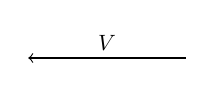
\begin{tikzpicture}
  \draw[->] (2,0)-- (0,0) node[pos=0.5,above,scale=0.8] {$V$};
  \end{tikzpicture}
  %%%%%%%%%%%%%%%%%%%%%%%%%%
  \caption{Local relations for colored graphs.
           Here $\ph\circ\psi$ is defined by \eqref{e:composition}.
          }\label{f:local_rels1}
\end{figure}

    Local relations should be understood as follows: for any pair
    $\Ga, \Ga'$ of colored graphs which are identical outside a subdisk
	$D'\subset D$, and in this disk are homeomorphic to the graphs
    shown in \firef{f:local_rels1}, we must have $\<\Ga\>=\<\Ga'\>$.
   \end{enumerate}
% Moreover, so defined $\<\Ga\>$ satisfies the following properties:
% \begin{enumerate}
% \item $\<\Ga\>$ is linear in color of each vertex $v$ (for
% fixed colors of edges and other vertices).
% \item $\<\Ga\>$ is additive in colors of edges as shown in
% \firef{f:linearity}.
%\begin{figure}[ht]
%$$
%%%%%%%%%%%%%
%\begin{tikzpicture}
%\node[morphism] (ph) at (0,0) {$\ph$};
%\node[morphism] (psi) at (1.5,0) {$\psi$};
%\node at (-0.7,0.1) {$\vdots$};
%\node at (2.2,0.1) {$\vdots$};
%\draw[->] (ph)-- +(220:1cm) node[pos=1.0,below,scale=0.8] {$V_n$};
%\draw[->] (ph)-- +(140:1cm) node[pos=1.0,above,scale=0.8] {$V_1$};
%\draw[->] (psi)-- +(40:1cm) node[pos=1.0,above,scale=0.8] {$W_m$};
%\draw[->] (psi)-- +(-40:1cm) node[pos=1.0,below,scale=0.8] {$W_1$};
%\draw[->] (ph) -- (psi) node[pos=0.5,above,scale=0.8] {$X_1\oplus X_2$};
%\end{tikzpicture}
%%%%%%%%%%%%%
%=
%%%%%%%%%%%%%
%\begin{tikzpicture}
%\node[morphism] (ph) at (0,0) {$\ph_1$};
%\node[morphism] (psi) at (1.5,0) {$\psi_1$};
%\node at (-0.7,0.1) {$\vdots$};
%\node at (2.2,0.1) {$\vdots$};
%\draw[->] (ph)-- +(220:1cm) node[pos=1.0,below,scale=0.8]{$V_n$};
%\draw[->] (ph)-- +(140:1cm) node[pos=1.0,above,scale=0.8]{$V_1$};
%\draw[->] (psi)-- +(40:1cm) node[pos=1.0,above,scale=0.8]{$W_m$};
%\draw[->] (psi)-- +(-40:1cm) node[pos=1.0,below,scale=0.8]{$W_1$};
%\draw[->] (ph) -- (psi) node[pos=0.5,above,scale=0.8] {$X_1$};
%\end{tikzpicture}
%%%%%%%%%%%%%
%+
%%%%%%%%%%%%%
%\begin{tikzpicture}
%\node[morphism] (ph) at (0,0) {$\ph_2$};
%\node[morphism] (psi) at (1.5,0) {$\psi_2$};
%\node at (-0.7,0.1) {$\vdots$};
%\node at (2.2,0.1) {$\vdots$};
%\draw[->] (ph)-- +(220:1cm) node[pos=1.0,below,scale=0.8]{$V_n$};
%\draw[->] (ph)-- +(140:1cm) node[pos=1.0,above,scale=0.8]{$V_1$};
%\draw[->] (psi)-- +(40:1cm) node[pos=1.0,above,scale=0.8]{$W_m$};
%\draw[->] (psi)-- +(-40:1cm) node[pos=1.0,below,scale=0.8]{$W_1$};
%\draw[->] (ph) -- (psi) node[pos=0.5,above,scale=0.8] {$X_2$};
%\end{tikzpicture}
%%%%%%%%%%%%%
%$$
%\caption{Linearity of $\<\Ga\>$. Here $\ph_1,\ph_2$ are compositions
%of $\ph$ with projector $X_1\oplus X_2\to X_1$ (respectively,
%$X_1\oplus X_2\to X_2$), and similarly for $\psi_1,\psi_2$.
%}\label{f:linearity}
%\end{figure}
%
% \item If $\Ga,\Ga'$ are two isomorphic colorings of the same graph,
% then $\<\Ga\>=\<\Ga'\>$.
% \item Composition property: if $D'\subset D$ is a subdisk such
% that $\del D'$ does not contain vertices of $\Ga$ and meets edges of
% $\Ga$ transversally, then $\<\Ga\>_D$ will not change if we replace
% subgraph $\Ga\cap D'$ by a single vertex colored by
% $\<\Ga\cap D'\>_{D'}$.
%
% \end{enumerate}
We will call the vector $\<\Ga\>$ the {\em evaluation} of $\Ga$.
\end{theorem}

In particular, for a closed $\calC$-colored graph $\Ga\subset \R^2$,
$\<\Ga\>\in \kk$ is a number.

The evaluation map $\Ga\to\<\Ga\>$ defined in \thref{t:evaluation-disk} has a
number of useful properties which can be found, e.g., in
\ocite{kirillov-stringnet}. We only give here one of them.

\begin{lemma}\label{l:eval-subdisk}
  Let $\Ga$ be a $\calC$-colored graph in a disk $D$, and let $D'\subset D$ be
  a subdisk such that $\del D'$ does not contain vertices of $\Ga$ and meets
  edges of $\Ga$ transversally. Then $\<\Ga\>_D$ will not change if we replace
  subgraph $\Ga\cap D'$ by a single vertex colored by $\<\Ga\cap D'\>_{D'}$.
\end{lemma}

Moreover, it turns out that we can also define $\<\Ga\>$ for a $\calC$-colored
graph on the sphere.

\begin{lemma}\label{l:colored-spherical}
  Let $\Ga$ be a $\calC$-colored graph on the sphere $S^2$. Choose a point $p\in
  S^2$ which does not lie on any of the edges of $\Ga$; then we can
  identify $S^2\setminus\{p\}\simeq \R^2$ and thus define
  $\<\Ga\>_{S^2\setminus\{p\}}\in \kk$.

  Then so-defined $\<\Ga\>_{S^2\setminus\{p\}}$ does not depend on the choice
  of point
  $p$.
\end{lemma}
Indeed, it suffices to show that the number $\<\Ga\>_{S^2\setminus\{p\}}$ does
not
change when we move point $p$ through one of the edges of $\Ga$. But this is
exactly the equality of left and right traces in \deref{d:spherical}:

$$
\begin{tikzpicture}[vcenter]
      \node[morphism_sq] (f) at (0,0) {$f$};
      \draw(f.north)-- +(0, 0.3) coordinate (top1)
            arc (180:0:0.5) coordinate (top);
      \draw(f.south)-- +(0, -0.3) coordinate (bot1)
            arc (-180:0:0.5)
      coordinate (bottom);
      \draw(top)--(bottom);
      %\node[right] at (top) {$X^*$};
      %\node[left] at (top1) {$X$};
      %\node[left] at (bot1) {$X^{**}$};
  \end{tikzpicture}
\qquad = \qquad
  \begin{tikzpicture}[vcenter]

      \node[morphism_sq] (f) at (0,0) {$f$};
      \draw(f.north)-- +(0, 0.3) coordinate (top1)
            arc (0:180:0.5) coordinate (top);
      \draw(f.south)-- +(0, -0.3) coordinate (bot1)
            arc (0:-180:0.5)
      coordinate (bottom);
      \draw(top)--(bottom);
      %\node[left] at (top) {$X^*$};
      %\node[right] at (top1) {$X^{**}$};
      %\node[right] at (bot1) {$X$};
    \end{tikzpicture}
$$

\leref{l:colored-spherical} was first proved in \ocite{barrett}; in fact, this
was the motivation for introducing the notion of a spherical category (which
also explains the name).

To simplify the future constructions, we introduce two additional conventions
for working with colored graphs.
\begin{convention}\label{c:summation_convention}
  If a colored graph contains a pair of
  vertices, one with outgoing edges labeled $A_1,\dots, A_n$ and
  the other with edges labeled $A_n^*,\dots, A_1^*$, and the vertices are
  labeled by a pair of letters $\ph,\ph^*$ (or $\psi, \psi^*$, or \dots),
  it will stand for summation over the dual bases:
  \begin{equation}\label{e:summation_convention}
    \begin{tikzpicture}[baseline=0pt]
      \node[morphism] (ph) at (0,0) {$\ph$};
      \draw[->] (ph)-- +(240:1cm) node[pos=0.7, left] {$A_n$} ;
      \draw[->] (ph)-- +(180:1cm);
      \draw[->] (ph)-- +(120:1cm);
      \draw[->] (ph)-- +(60:1cm);
      \draw[->] (ph)-- +(0:1cm);
      \draw[->] (ph)-- +(-60:1cm) node[pos=0.7, right] {$A_1$};
      %
      \node[morphism] (ph') at (3,0) {$\ph^*$};
      \draw[->] (ph')-- +(240:1cm) node[pos=0.7, left] {$A_1^*$} ;
      \draw[->] (ph')-- +(180:1cm);
      \draw[->] (ph')-- +(120:1cm);
      \draw[->] (ph')-- +(60:1cm);
      \draw[->] (ph')-- +(0:1cm);
      \draw[->] (ph')-- +(-60:1cm) node[pos=0.7, right] {$A_n^*$};
    \end{tikzpicture}
    \quad = \sum_\al\quad
    \begin{tikzpicture}[baseline=0pt]
      \node[morphism] (ph) at (0,0) {$\ph_\al$};
      \draw[->] (ph)-- +(240:1cm) node[pos=0.7, left] {$A_n$} ;
      \draw[->] (ph)-- +(180:1cm);
      \draw[->] (ph)-- +(120:1cm);
      \draw[->] (ph)-- +(60:1cm);
      \draw[->] (ph)-- +(0:1cm);
      \draw[->] (ph)-- +(-60:1cm) node[pos=0.7, right] {$A_1$};
      %
      \node[morphism] (ph') at (3,0) {$\ph^\al$};
      \draw[->] (ph')-- +(240:1cm) node[pos=0.7, left] {$A_1^*$} ;
      \draw[->] (ph')-- +(180:1cm);
      \draw[->] (ph')-- +(120:1cm);
      \draw[->] (ph')-- +(60:1cm);
      \draw[->] (ph')-- +(0:1cm);
      \draw[->] (ph')-- +(-60:1cm) node[pos=0.7, right] {$A_n^*$};
    \end{tikzpicture}
  \end{equation}
  where $\ph_\al\in \<A_1,\dots, A_n\>$, $\ph^\al\in \<A_n^*,\dots, A_1^*\>$
  are dual bases with respect to the pairing \eqref{e:dual}.
\end{convention}

\begin{convention}
  A dashed line in a colored graph will
  stand for the sum of all colorings of an edge by
  simple objects $i$, each taken with coefficient $d_i=\dim X_i$:
  \begin{equation} \label{e:regular_color}
    \begin{tikzpicture}[vcenter]
        \draw[regular] (0, -0.5)--(0, 0.5);
       \end{tikzpicture}
      \quad =\sum_{i\in\OC} d_i \quad
      \begin{tikzpicture}[vcenter]
        \draw (0, -0.5)--(0, 0.5) node[pos=0.8, right] {$i$};
       \end{tikzpicture}
   \end{equation}
\end{convention}

Using these conventions, we can formulate some properties of colored graphs.
\begin{lemma}\label{l:colored-graphs}
  We have the following equalities \textup{(}here and below, equality of two
  colored graphs should be understood as equality $\<\Ga_1\>=\<\Ga_2\>$\textup{)}:

  \begin{align}
  &\begin{tikzpicture}[vcenter]
    \draw[regular] (0,0) circle (0.5);
   \end{tikzpicture}
   \quad =\dim\calC\\
  & %%%%%%%%%%%%%%%
  \begin{tikzpicture}[vcenter]
    \node[morphism] (ph) at (0,-0.5) {$\al$};
    \node[morphism] (psi) at (0,0.5) {$\al^*$};
    \node at (0,1.3) {$\dots$};
    \node at (0,-1.3) {$\dots$};
    \draw[->] (ph)-- +(-110:1cm) node[pos=1.0,left,scale=0.8] {$A_1$};
    \draw[->] (ph)-- +(-70:1cm) node[pos=1.0,right,scale=0.8] {$A_n$};
    \draw[<-] (psi)-- +(110:1cm) node[pos=1.0,left,scale=0.8] {$A_1$};
    \draw[<-] (psi)-- +(70:1cm) node[pos=1.0,right,scale=0.8] {$A_n$};
    \draw[regular] (ph) -- (psi) node[pos=0.5,left,scale=0.8] {};
  \end{tikzpicture}
   %%%%%%%%%%%%%%%%%
    =
   %%%%%%%%%%%%%%%%%
    \begin{tikzpicture}[vcenter]
     \node at (0,0) {$\dots$};
     \draw[<-] (-0.3,-1)-- (-0.3,1) node[pos=0.5,left,scale=0.8] {$A_1$};
     \draw[<-] (0.3,-1)-- (0.3,1) node[pos=0.5,right,scale=0.8] {$A_n$};
    \end{tikzpicture}
    %%%%%%%%%%%%%%%%%%
  \end{align}
\end{lemma}
%%%%%%%%%%%%%%%%%%%%%%%%%%%%%%%%%%
\section{Canonical algebra}\label{s:canonical-alg}
For Frobenius algebras, non-degeneracy of the pairing $(\, , \,)$ also gave us
the coevaluation linear map $\coev\colon \kk\to A\otimes A$, or equivalently, an
element $e=\coev(1)=\sum x_i \otimes x^i \in A\otimes A$. Again, it has an
obvious analog for spherical fusion categories.

\begin{lemma}\label{l:spherical-E}
  Let $\calC$ be a spherical fusion category. Let
  \begin{equation}\label{e:spherical-E}
    E = \bigoplus_{i\in \OC} X_i\boxtimes X_i^*\in \calC\boxtimes\calC.
  \end{equation}
  Then we have the following properties:
  \begin{enumerate}
    \item So defined $E$ is independent of the choice of representatives of
    isomorphism classes of simple objects: different choices give canonically
    isomorphic objects $E$.

    \item It is symmetric: there is an isomorphism $c\colon E\simeq P(E)$, where
    $P \colon \calC\boxtimes\calC \to \calC\boxtimes \calC$ is given by
    $P(X\boxtimes Y)= Y\boxtimes X$, and $c^2=1$.

    \item For any $X\in \calC$, we have a canonical functorial isomorphism
    $$
      X \simeq \bigoplus_i\<X, X_i\>\otimes X_i^*
    $$
  \end{enumerate}
\end{lemma}
 The proof  is straightforward; details can be found, e.g.,
  in \ocite{balsam-kirillov}.
\begin{remark}
  If we consider $E$ as an object in $\calC\boxtimes\calC^\mop$, then one can
  show that it has a canonical structure of an algebra in that category; this
  algebra is sometimes called the \emph{canonical algebra} of $\calC$, see
  \ocite{etingof-fusion}*{Example 7.9.14}, where it is shown that $E\simeq
  \underline{\Hom}(\one,\one)$, where $\underline{\Hom}$ is the so-called inner
  hom.
\end{remark}

We also have an analog of bicentrality (compare with \leref{l:bicentral}).
\begin{lemma}\label{l:cat-bicentral}
  Let $\calC$ be a spherical fusion categor, and let $E\in \calC\boxtimes\calC$
  be defined by \eqref{e:spherical-E}. Then $E$ is bicentral:
  for any $A\in \calC$, we have canonical
  functorial isomorphisms
    \begin{align*}
      \ga_A\colon \bigoplus (A\otimes X_i) \boxtimes X_i^* &\simeq
        \bigoplus X_i \boxtimes (X_i^* \otimes A)\\
      \ga'_A\colon \bigoplus (X_i\otimes A) \boxtimes X_i^* &\simeq
          \bigoplus X_i \boxtimes (A\otimes X_i^*)
    \end{align*}
    which satisfy
    $$
      \ga_{A\otimes B} =(\ga_A\otimes 1_B)\circ (1_A\otimes \ga_B).
    $$
    and similarly for $\ga'$.
\end{lemma}
\begin{proof}
  We define the isomorphism $\ga$ by the following picture:
  \begin{equation}\label{e:gamma}
    \ga_A = \bigoplus_{i,j\in \OC} d_i
    \begin{tikzpicture}[baseline=0pt]
      \coordinate (bot) at (0,-1.5);
      \coordinate (top) at (0,1.5);
      \node at (0,0) {$\boxtimes$};
      \node[morphism] (al) at (-0.7,0) {$\al$};
      \node[morphism] (al*) at (0.7,0) {$\al$};
      \draw[->] (al) -- (al|-bot) node[pos=0.8,right] {$j$};
      \draw[->] (al|-top) -- (al) node[pos=0.1,right] {$i$};
      \draw[<-] (al.120) to[out=120, in =-90] (-1.2,1.5);
      \node[below left] at (-1.2,1.5){$A$};
      \draw[->] (al*|-bot) -- (al*) node[pos=0.1,right] {$j$};
      \draw[->] (al*) -- (al*|-top) node[pos=0.8,right] {$i$};
      \draw[out=-60, in=90,->] (al*.-60) to (1.2,-1.5);
      \node[above right] at (1.2,-1.5) {$A$};
    \end{tikzpicture}
  \end{equation}
  We refer the reader to \ocite{balsam-kirillov} for the proof that so defined
  $\ga$ satisfies $\ga_{A\otimes B}=\ga_A\circ \ga_B$;
  another proof of centrality of $E$ is given in
  \ocite{etingof-fusion}*{Proposition 7.18.5}.

  Construction of isomorphism $\ga'$ is similar and is left to the reader.
\end{proof}

Note that both the symmetry of $E$ and bicentrality use pivotal structure;
 without the pivotal structure, these result need some changes.
\begin{exercise}\label{ec:E-nonpivotal}
  Let  $\calC$ be a fusion category (not necessary pivotal), and let $E$ be
  defined by \eqref{e:spherical-E}.
  \begin{enumerate}
    \item Show that $P(E)\simeq (D \otimes 1)E \simeq (1\otimes D^{-1})E$,
      where functor $D\colon  \calC\to\calC$ is given by $D(X)=X^{**}$.
    \item Use pairing defined in \reref{r:pairing-nonpivotal} to construct
      functorial isomorphisms
    \begin{align*}
      \ga_A\colon \bigoplus (A\otimes X_i) \boxtimes X_i^* &\simeq
        \bigoplus X_i \boxtimes (X_i^* \otimes A^{**})\\
      \ga'_A\colon \bigoplus (X_i\otimes A) \boxtimes X_i^* &\simeq
          \bigoplus X_i \boxtimes (A\otimes X_i^*)
    \end{align*}
    (note $A^{**}$ in the first isomorphism!)
  \end{enumerate}
\end{exercise}
%%%%%%%%%%%%%%%%%%%%%%%%%%%%%%%%%%
\section{Drinfeld center}\label{s:drinfeld-center}
For an associative algebra $A$, we can define its center $z(A)$ (which is a
commutative algebra) and $A/[A,A]$, which is just a vector space. Both
constructions played an important role in the construction of extended 2d TQFTs; in
particular, we have shown that for a separable symmetric Frobenius algebra one
has a natural map $A\to z(A)\colon a\mapsto \sum x_iax^i$, which descends to an
isomorphism $A/[A,A]\simeq z(A)$.

In this section, we define similar notions for a spherical fusion category,
starting with the categorical analog of the center, which in this case is
called the \emph{Drinfeld center}. Our exposition
follows \ocite{etingof-fusion}*{Section 7.13}.
\begin{definition}\label{d:drinfeld-center}
  Let $\calC$ be a monoidal category. Its \emph{Drinfeld center}\index{Drinfeld
  center} is the category $\calZ(\calC)$ with the following objects and
  morphisms:
  \begin{itemize}
    \item Objects: pairs $(Z, \ga)$, where $Z\in \calC$ and $\ga$ is a functorial
    isomorphism
    $$
      \ga_A\colon A\otimes Z\to Z\otimes A
    $$
    satisfying the following conditions:
    \begin{enumerate}
      \item Hexagon axiom: the following diagram is commutative:

      \begin{equation}\label{e:hexagon-drinfeld}
        \begin{tikzcd}[column sep=5mm, row sep=large]
          A\otimes B\otimes Z
          \arrow[rr,"\ga_{A\otimes B}"]
          \arrow[dr,"1_A\otimes \ga_B"']
          && Z\otimes A\otimes B\\
          & A\otimes Z\otimes B
          \arrow[ur,"\ga_A\otimes 1_B"] &
        \end{tikzcd}
      \end{equation}
      (For better readability, we have dropped associativity isomorphisms
      from this diagram; compare with hexagon axiom in \deref{d:symmetric}.)


      \item Triangle axiom: $\ga_\one\colon \one \otimes Z\to Z\otimes \one$
      coincides with composition of unit isomorphisms $\one\otimes Z\simeq
      Z\simeq Z\otimes \one$.
    \end{enumerate}
    $\ga$ is usually called the \emph{half-braiding}.
    \item Morphisms:
    $$
    \Hom_{\calZ(\calC)}((Z, \ga), (Z', \ga'))
      =\{f \in \Hom_\calC(Z,Z')\st \ga' (1 \otimes f) =(f\otimes 1) \ga\}.
    $$
  \end{itemize}
\end{definition}



\begin{example}\label{x:center-vectg}
  Let $\vect_G$ be the category of $G$-graded vector spaces. Then an object
  of $\calZ(\vect_G)$ is a $G$-graded vector space together with a collection
  of isomorphisms $V_{gh}\simeq V_{hg}$ for any $g$. Equivalently, it is a
  $G$-graded vector space together with an action of $G$ such that
  $$
   gV_h\subset V_{ghg^{-1}}.
  $$
  This can also be described as a category of representations of algebra
  $A=\kk(G)\# \kk[G]$, where $\kk(G)$ is the algebra of functions on $G$
  with pointwise multiplication, $\kk[G]$ is the group algebra, and $\#$ is
  the smash product (also called the cross product) of algebras with
  respect to natural action of $\kk[G]$ on $\kk(G)$.
\end{example}
More generally, it can be shown that for $\calC=\Rep H$, where $H$ is a
finite-dimensional Hopf algebra, $\calZ(\Rep H)$ is equivalent to the
representation category of a new Hopf algebra $D(H)$, called the \emph{Drinfeld
double}\index{Drinfeld double} of $H$. The algebra $D(H)$ contains both $H$ and
$H^*$ as subalgebras, and as a vector space, $D(H)\simeq H\otimes H^*$; however,
$H$ and $H^*$ do not commute in $D(H)$, so multiplication in $D(H)$ is
non-trivial. We refer the reader to \ocite{etingof-fusion}*{Section 7.14} for
details.

\begin{lemma}\label{l:drinfeld-monoidal}
  Let $\calC$ be a monoidal category.
  \begin{enumerate}
    \item $\calZ(\calC)$ has a natural structure of a monoidal category; if
      $\calC$ is rigid, so is $\calZ(\calC)$.
    \item If $\calC$ is a $\kk$-linear category, then $\calZ(\calC)$ is also
      a $\kk$-linear category.
    \item If $\calC$ is a pivotal \textup{(}respectively, spherical\textup{)} category, then
      $\calZ(\calC)$ is also pivotal \textup{(}respectively, spherical\textup{)}.
  \end{enumerate}
\end{lemma}
The proof is mostly straightforward; details can be fond in
\ocite{etingof-fusion}*{Section 7.13}.

\begin{lemma}\label{l:dr-center-2}
  Let $\calC$ be a finite tensor category. Then one has an equivalence of
  $\kk$-linear categories
  \begin{align*}
    \Fun_{\calC^e}(\calC, \calC)&\simeq \calZ(\calC)\\
                              F&\mapsto F(\one),
  \end{align*}
  where $\calC^e=\calC\boxtimes\calC^{\mop}$.
\end{lemma}
The proof is again a straightforward comparison of the definitions; see details
in  \ocite{etingof-fusion}*{Proposition 7.13.8}.


\begin{theorem}\label{t:drinfeld-fusion}
  The Drinfeld center of a fusion category is itself a fusion category.
\end{theorem}
\begin{proof}
  Indeed, by \leref{l:drinfeld-monoidal}, $\calZ(\calC)$ is a rigid monoidal
  $\kk$-linear  category, and the  unit object of $\calZ(\calC)=\one$ is
  simple. Thus, it only remains to show that $\calZ(\calC)$ is finite and
  semisimple. This  immediately follows from \leref{l:dr-center-2} together
  with \thref{t:module-functors}
\end{proof}

\begin{theorem}\label{t:drinfeld-dim}
  Let $\calC$ be a spherical fusion category. Then $\calZ(\calC)$ is also a
  spherical fusion category, and
  $$
    \dim \calZ(\calC) = (\dim \calC)^2.
  $$
\end{theorem}
See \ocite{etingof-fusion}*{Proposition 9.3.4}.
\begin{remark}\label{r:drinfeld-size}
  This shows that contrary to naive intuition, the Drinfeld center  of $\calC$
  is ``larger'' than $\calC$ (at least, has larger dimension). In particular,
  $$
  \Gr(\calZ(\calC))\ne z(\Gr(\calC)).
  $$
   Note that in general, it is very hard to describe all simple objects in
   $\calZ(\calC)$, even knowing all simple objects of $\calC$.
\end{remark}

Since every object of $\calZ(\calC)$ is also an object of $\calC$, it is easy
to extend our graphical calculus, allowing $\calC$-colored graphs where some
arcs are colored by objects of $\calZ(\calC)$. In these graphs, we
will show objects of $\calZ(\calC)$ by double green lines and the
half-braiding isomorphism $\ga_A\colon A\otimes Z\to Z\otimes A$ by a
crossing as in \firef{f:crossing}.
\begin{figure}[ht]
  \begin{tikzpicture}[baseline=0pt]
    \draw[drinfeld center](0,0)--(1cm,2cm) node [pos=0.2, left,black] {$Z$};
    \draw[overline](1cm,0) -- (0,2cm) node [pos=0.2, right] {$A$};
  \end{tikzpicture}

  \caption{Graphical presentation of the half-braiding
    $\ga_A\colon A\otimes Z\to Z\otimes A$,
    $A\in \calC$, $Z\in \calZ(\calC)$ }\label{f:crossing}
\end{figure}


\begin{exercise}\label{ec:drinfeld-hexagon}
  Show that for any morphism $\ph \colon A_1\otimes \dots\otimes A_k\to
  B_1\otimes\dots \otimes B_m$ in $\calC$, we have the following equality:
  $$
    \begin{tikzpicture}[vcenter]
        %% drinfeld center
        \node[label=above:$Z$] (z) at (-1,1.5) {};
        \draw[drinfeld center] (z) to [out=-90, in=90] (1,0)-- (1,-1);
        %% morphism
       \node[morphism_sq, minimum width=1.4cm] (ph) at (0,0) {$\ph$};
        %% top
        \node[label=above:$A_1$] (A1) at (-0.4,1.5){};
        \node[label=above:$A_k$] (Ak) at (0.4,1.5){};
        \node at (0, 1.1) {\dots};
        \draw[overline] (A1)-- (A1|-ph.north);
        \draw[overline] (Ak)-- (Ak|-ph.north);
        %% bottom
        \node[label=below:$B_1$] (B1) at (-0.4,-1){};
        \node[label=below:$B_m$] (Bm) at (0.4,-1){};
        \node at (0, -0.6) {\dots};
        \draw[] (B1)-- (B1|-ph.south);
        \draw[] (Bm)-- (Bm|-ph.south);
    \end{tikzpicture}
    \quad = \quad
    \begin{tikzpicture}[vcenter]
        %% drinfeld center
        \node[label=above:$Z$] (z) at (-1,1) {};
        \draw[drinfeld center] (z) -- (-1,0) to [out=-90, in=90]
        (1,-1.5);
        %% morphism
       \node[morphism_sq, minimum width=1.4cm] (ph) at (0,0) {$\ph$};
        %% top
        \node[label=above:$A_1$] (A1) at (-0.4,1){};
        \node[label=above:$A_k$] (Ak) at (0.4,1){};
        \node at (0, 0.6) {\dots};
        \draw[overline] (A1)-- (A1|-ph.north);
        \draw[overline] (Ak)-- (Ak|-ph.north);
        %% bottom
        \node[label=below:$B_1$] (B1) at (-0.4,-1.5){};
        \node[label=below:$B_m$] (Bm) at (0.4,-1.5){};
        \node at (0, -1.1) {\dots};
        \draw[overline] (B1)-- (B1|-ph.south);
        \draw[overline] (Bm)-- (Bm|-ph.south);
    \end{tikzpicture}
  $$
\end{exercise}

\begin{exercise}\label{ec:drinfeld-projector}
  Let $\calC$ be a spherical fusion category and let
  $(Z,\ga)$, $(Z', \ga')$ be two objects of $\calZ(\calC)$. Define a map
  $P\colon \Hom_\calC(Z,Z')\to \Hom_\calC(Z,Z')$ (note that at the moment we
  are not requiring any compatibility with half-braidings $\ga, \ga'$) by the
  graph below:
  \begin{equation}
  P(f) = \frac{1}{\dim \calC}\quad
    \begin{tikzpicture}[vcenter]
       \node[morphism_sq] (f) at (0,0) {$f$};
       \draw[drinfeld center] (f)-- +(0,1.2) node[black,left] {$Z$};
       \draw[drinfeld center] (f)-- +(0,-1.2) node[black,left] {$Z'$};
       \draw[regular, overline] (f) circle (0.6);
    \end{tikzpicture}
  \end{equation}
  Use \leref{l:colored-graphs} to
  prove that then $P$ is a projector onto
  $\Hom_{\calZ(\calC)}(Z,Z')\subset \Hom_\calC(Z,Z')$.
\end{exercise}




Finally, note that for algebras, we had a natural embedding $z(A)\subset A$ and
also the map $A\to z(A)\colon a \mapsto \sum x_iax^i$. These two maps are not inverses
of each other; their composition is multiplication by the Euler element
$w=\sum x_ix^i$.

Similar constructions exist for categories.
Namely, we have the obvious forgetful functor
\begin{equation}
  \begin{aligned}
    F\colon \calZ(\calC)&\to \calC\\
    (Z,\ga)&\mapsto Z.
  \end{aligned}
\end{equation}

\begin{theorem}\label{t:drinfeld-induction}
  Let $\calC$ be a spherical fusion category. Then
  the forgetful functor $F$ has a left adjoint functor
  $$
    I\colon \calC\to \calZ(\calC)
  $$
  given by
  $$
    I(V)=\bigoplus_{i\in \OC} X_i\otimes V \otimes X_i^*
  $$
  with $\ga$ given by:
  \begin{equation}\label{e:gamma2}
    \ga_A = \bigoplus_{i,j\in \OC} d_i
    \begin{tikzpicture}[baseline=0pt]
      \coordinate (bot) at (0,-1.5);
      \coordinate (top) at (0,1.5);
      \draw[->] (top)--(bot);
      \node[above] at (0,1.5) {$V$};
      \node[morphism] (al) at (-0.7,0) {$\al$};
      \node[morphism] (al*) at (0.7,0) {$\al^*$};
      \draw[->] (al) -- (al|-bot) node[pos=0.8,right] {$j$};
      \draw[->] (al|-top) -- (al) node[pos=0.1,right] {$i$};
      \draw[<-] (al.120) to[out=120, in =-90] (-1.2,1.5);
      \node[below left] at (-1.2,1.5){$A$};
      \draw[->] (al*|-bot) -- (al*) node[pos=0.1,right] {$j$};
      \draw[->] (al*) -- (al*|-top) node[pos=0.8,right] {$i$};
      \draw[out=-60, in=90,->] (al*.-60) to (1.2,-1.5);
      \node[above right] at (1.2,-1.5) {$A$};
    \end{tikzpicture}
  \end{equation}
  \textup{(}compare with \eqref{e:gamma}\textup{)}.
\end{theorem}
We refer the reader to \ocite{balsam-kirillov}*{Theorem 2.3} for the proof.

Note that this implies that any object $Z\in \calZ(\calC)$ is a direct summand
of an object of the form $I(A)$, $A\in \calC$: we can take $A=F(Z)$.

%%%%%%%%%%%%%%%%%%%%%%%%%%%
\section{Center and universal trace}\label{s:cat-trace}
Recall from \seref{s:invariants} that for a bimodule $M$ over an associative
algebra $A$, we defined the spaces of invariants and coinvariants by
\begin{equation}
  \begin{aligned}
    M^{A}&=\Hom(A,M)=\{m\in M\st am=ma \text{ for any } a\in A\}\\
    M_{A}&=A\otimes_{A^e} M = M/\<am-ma\>
  \end{aligned}
\end{equation}
where $\Hom$ is computed in the category of $A$-bimodules, or equivalently,
modules over $A^e=A\otimes A^\op$. In particular, for $M=A$, these definitions
give
\begin{align*}
  HH^0(A)&=A^{(A)}=z(A),\\
  HH_0(A)&=A_{(A)}= A/[A,A].
\end{align*}

It is natural to ask if we can define an analog of this for a bimodule category
$\calM$ over a finite tensor category $\calC$. In the previous section, we have
already given an answer in the special case $\calM=\calC$, defining the Drinfeld
center $\calZ(\calC)$, which is an analog of $z(A)$. In this section we
consider the more general case. Our exposition follows
\ocite{fuchs-schaumann-schweigert-trace}; other references for the material of
this section include \ocite{greenough} (probably one of the earliest references
on this topic) and \ocite{benzvi-francis-nadler}*{Section 5} (in the context
of $\infty$-categories).

\begin{definition}\label{d:cat-center}
  Let $\calM$ be a finite bimodule category over a finite tensor category
  $\calC$. Define the \emph{categorical center}\index{categorical center}
  $\calZ(\calM)$ as the category
  with the following objects and morphisms:
    \begin{itemize}
      \item Objects: pairs $(M, \ga)$, where $M\in \calM$ and $\ga$ is a
      functorial isomorphism
      $$
        \ga_A\colon A\otimes M\to M\otimes A, \quad A\in \calC,
      $$
      satisfying the hexagon and unit axioms similar to those in
      \deref{d:drinfeld-center}.
      \item Morphisms:
      $$
      \Hom_{\calZ(\calM)}((M, \ga), (M', \ga'))
        =\{f \in \Hom_\calM(M,M')\st \ga' (1 \otimes f) =(f\otimes 1) \ga\}.
      $$
    \end{itemize}
  \end{definition}

\begin{lemma}\label{l:cat-center-functor}
  Under the assumptions of \deref{d:cat-center},
  one has an equivalence of categories
  \begin{align*}
  \Fun_{\calC^e}(\calC, \calM)&\simeq\calZ(\calM)\\
    F&\mapsto F(\one)
  \end{align*}
\end{lemma}

As an immediate corollary, we see that $\calZ(\calM)$ is a finite $\kk$-linear
category; one can show (FIXME) that if $\calM$ is semisimple, then so is
$\calZ(\calM)$.

Let us now try to define the analog of coinvariants $M_A$. For bimodules over
an algebra, we had defined $M_A=M/\<am-ma\>$. A better way to define $M_A$ is
by using the universal property: for any vector space $L$,
$$
  \Hom(M_A,L)=\Bal(M,L)
$$
where $\Bal$ stands for the space of balanced maps, i.e., maps $f\colon M\to L$
satisfying the condition
$$
  f(am)=f(ma), \quad a\in A.
$$
We can now define an analog of this for bimodule categories. First, we define an
analog of balanced maps, essentially in the same way as we did in
\seref{s:balanced-product} when defining the balanced Deligne product of
categories.

\begin{definition}\label{d:balanced2}
  Let $\calM$ be a bimodule category over a finite tensor category $\calC$,
  and let $\calL$ be a $\kk$-linear category. A $\calC$-balanced functor
  $\calM\to\calL$ is a pair $(F,J)$, where $F\colon \calM\to\calL$ is a
  $\kk$-linear right exact functor, and $J$ is a functorial isomorphism
  $$
    J\colon F(C\otimes M)\simeq F(M\otimes C), \quad M\in \calM, C\in \calC
  $$
  satisfying the obvious compatibility conditions (compare with
  \deref{d:balanced}).
\end{definition}

One can also define a notion of morphisms of $\calC$-balanced functors. We
denote by $\Bal_\calC(\calM, \calL)$ the category of
$\calC$-balanced functors $\calM\to \calL$.


\begin{definition}\label{d:cat-trace}
  Under the assumptions of \deref{d:balanced2}, a categorical trace is a
  $\kk$-linear category $\circtensor\calM$ together with a
  $\calC$-balanced functor $F\colon \calM\to \circtensor \calM$
  such that for any $\kk$-linear category
  $\calL$, functor $F$ induces an equivalence of categories
  $$
    \Bal_\calC(\calM, \calL)\simeq
    \Fun(\circtensor \calM, \calL).
  $$
\end{definition}

As with the definition of the balanced tensor product, it is easy to show that
$\circtensor \calM$, if it exists, is unique up to a unique equivalence. However,
existence is not obvious.

\begin{example}\label{x:trace-deligne-product}
  Let $\calM_\calC$, ${}_\calC \calN$ be right and left finite module
  categories over $\calC$. Then Deligne's product $\calM\boxtimes \calN$ is
  a $\calC$-bimodule category, and $\circtensor (\calM\boxtimes \calN)\simeq
  \calM\boxtimes_\calC\calN$; thus, in this case the existence of the balanced product
  (\thref{t:deligne-balanced}) implies the existence of the categorical trace
  $\circtensor (\calM\boxtimes\calN)$.
\end{example}
\begin{theorem}\label{t:cat-trace}
  Let $\calM$ be a finite bimodule category over a finite tensor category
  $\calC$. Then the categorical trace $\circtensor \calM$ exists;
  moreover, we have an equivalence of categories
  $$
    \calC\boxtimes_{\calC^e} \calM \simeq \circtensor \calM
  $$
  where, as before, $\calC^e=\calC\boxtimes\calC^\mop$.
\end{theorem}
  A proof of this theorem can be found in
  \ocite{fuchs-schaumann-schweigert-trace}*{Theorem 3.3}.


Finally, recall that for a module over a separable symmetric Frobenius algebra,
one has isomorphism $M_{(A)}\simeq M^{(A)}$ given by $m\mapsto \sum x_imx^i$,
see \seref{l:coinv-separable}. The following theorem is a categorical analog of
this statement.

\begin{theorem}\label{t:category-inv-coinv}
  Let $\calM$ be a finite bimodule category over a pivotal fusion
  category  $\calC$. Let functor $I\colon \calM\to \calZ(\calM)$ be defined by
  \begin{equation}
    I(M)= \bigoplus X_i\otimes M\otimes X_i^*
  \end{equation}
  with the half-braiding on $I(M)$ defined in the same way as in
  \thref{t:drinfeld-induction}.

  Then $I$ has a natural structure of a balanced functor, and it
  gives an equivalence of categories $\calZ(\calM)\simeq \circtensor \calM$.
\end{theorem}
\begin{proof}
    FIXME

    Balancing structure is given by functorial isomorphism
    $$
    \ga'_A\colon \bigoplus (X_i\otimes A) \boxtimes X_i^* \simeq
              \bigoplus X_i \boxtimes (A\otimes X_i^*)
    $$
    defined in \leref{l:cat-bicentral}.
\end{proof}